\section{ClickNP Language}
\label{clicknp:sec:language}

\subsection{Element Graph}

The ClickNP script defines a directed graph of elements and channels, which adapts some syntax from the Click modular router \cite{kohler2000click}.

The following ClickNP script and figure \ref{clicknp:fig:ClickNPScriptExample} define the network card-to-ToR part of a network application with NVGRE encapsulation and Per-VM rate limiting.

\begin{figure}[!t]
	\centering
	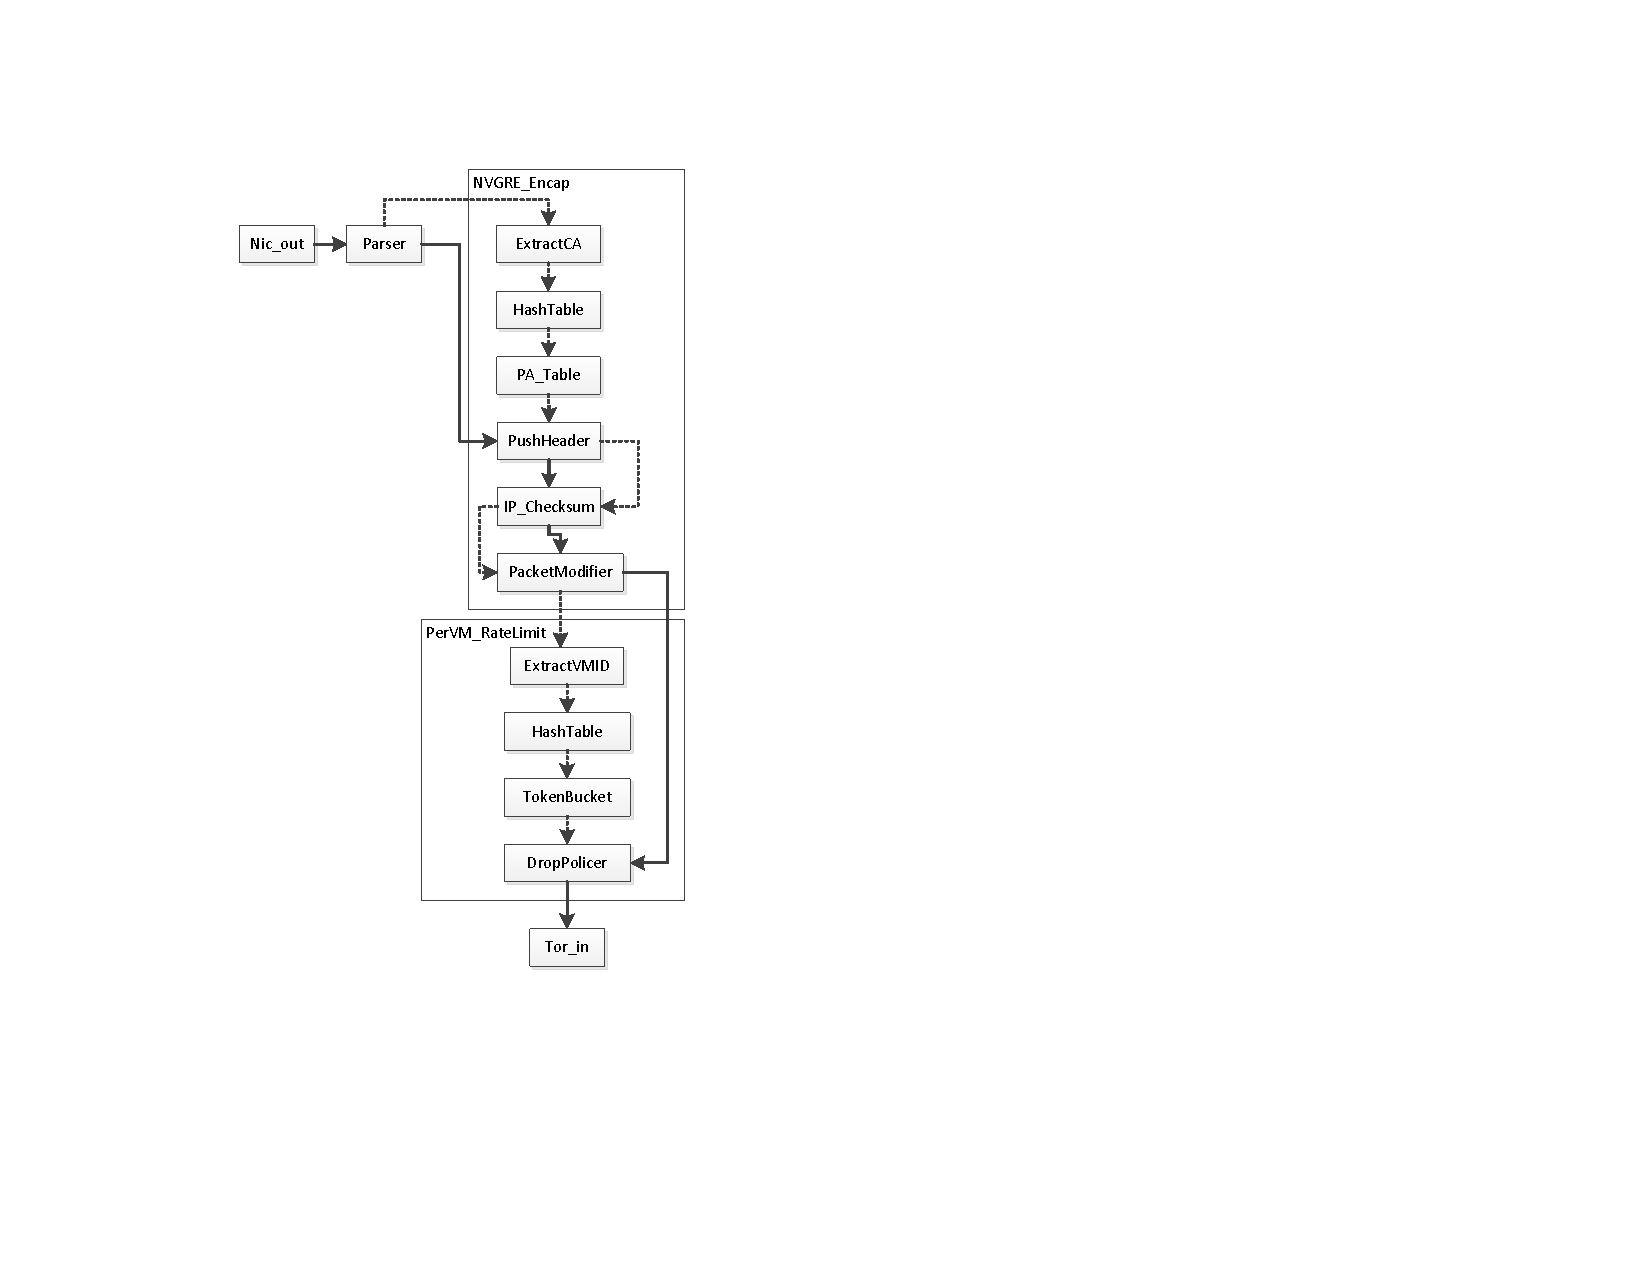
\includegraphics[width=1.0\columnwidth]{image/ApplicationExample}
	\vspace{-0.25in}
	\caption{NVGRE Encap + Rate Limiting in ClickNP}
	\vspace{-0.15in}
	\label{clicknp:fig:ClickNPScriptExample}
	%    
\end{figure}

\begin{lstlisting}
.element_group NVGRE_Encap {
    PushHeader :: encap (2,2)
    begin[1] -> [1]encap -> IP_Checksum (2,2) -> PacketModifer (2,2) -> end
    begin[2] -> ExtractCA (1,1) -> HashTable @ (1,1,14) -> PA_Table @ (1,1) -> [2]encap
}
.element_group PerVM_RateLimit {
    DropPolicer :: action (2,2)
    begin[1] -> [1]action -> end
    begin[2] -> ExtractVMID (1,1) -> HashTable @ (1,1,4) -> TokenBucket @ (1,1) -> [1]action
}
PerVM_RateLimit :: ratelimit (2,2)
nic_out -> Parser (1,2) -> NVGRE_Encap (2,2) -> ratelimit[1] -> tor_in
ratelimit[2] -> Drop (1,0)
\end{lstlisting}

Per clock cycle, each element can read at most one 64-byte message from each input channel and write zero or one 64-byte message to each output channel. A channel either passes \textit{flit} messages (solid line) or \textit{metadata} messages (dotted line). Each flit contains 32 bytes of packet content and flags indicating the start of a packet (sop) and the end of a packet (eop). The metadata format is user-defined, containing the parsed packet header and optionally a subsequent action.

Lines 1--5 define an \textit{element group} of 6 elements. Line 2 instantiates a \textit{PushHeader} element with the name \textit{encap}. Numbers in parentheses stand for the number of input and output ports, and optional subsequent numbers are element parameters (see section \ref{clicknp:subsec:elementdef}). Square brackets indicate the port number to be connected via channel. The ``@'' symbol indicates on-the-fly host control.

The metadata, which includes parsed packet headers, is directed into the element group via port 1. Here, the Customer Address (CA) is extracted and compared with a \textit{HashTable} that is controlled by the host program. The result of this comparison is then used as an index for the Physical Address (PA) table (also controlled by the host program). The PA table modifies the action part of the metadata to include the outer header offset, length, and data. The metadata, along with packet content flits stored in the channel, is sent to the \textit{PushHeader} element where the packets are actually shifted. The metadata (with the action cleared) and packet flits then proceed to the \textit{IP\_Checksum} element where a new IP header checksum is calculated and a packet modify action is generated to update the IP checksum field in the subsequent \textit{PacketModifier} element.

Our decision to separate flit and metadata messages was made not only for clarity but also for performance. One reason is to reduce the throughput load of lookup tables. Typically, table lookup is performed once per packet, while each Ethernet packet contains 2--48 flits. If flits are passed through via lookup tables, we can process at most one flit per cycle. To achieve line rate, we need to complete each iteration in one cycle, but lookup tables that both read and write to local memory require two cycles due to memory timing.

Another reason for separating flit and metadata is to pipeline packet modification actions. For instance, in the \textit{IP\_Checksum} action, the IP header spans the boundary of the first and second flits. Therefore, the checksum can only be calculated after the first two flits have arrived. However, the IP checksum field that needs to be updated is in the first flit. If we use one channel for both flit and metadata, then the element has to output nothing in the first cycle processing a packet. As discussed in section \ref{clicknp:subsec:designgoals}, such per-packet idle cycle is unacceptable for our line-rate FPGA implementation. By transferring flit and metadata in separate channels, the \textit{IP\_Checksum} element can pass through flits while calculating the checksum, and flits are buffered in the channel between the \textit{IP\_Checksum} and \textit{PacketModifier} elements. When the \textit{PacketModifier} receives the metadata containing the IP checksum, the first flit is also ready. This coding style eliminates the need for buffers within elements, which consume more resources than buffers within channels.

A network application is typically constructed with a parser and a sequence of network functions. A network function initially creates a lookup key from the parsed packet header, matches the key in a lookup table (section \ref{clicknp:subsec:lookuptables}), and then constructs an action based on the match result. The action and packet flits are subsequently passed into an action element. This coding convention allows lookup table elements to be generic, actions to be chained, network functions to be chained, and packet parser to be shared.

\subsection{Element Definition}
\label{clicknp:subsec:elementdef}

An element comprises five components: states, ports, an initializer, a data handler, and a signal handler.

\textit{States} delineate variables that persist throughout the element's lifecycle. Each element has several input and output \textit{ports}, the number of which is configured by the element graph. The \textit{Initializer} is executed once immediately after the element is launched. The main processing loop consists of a data handler (\textit{.handler}) and a signal handler (\textit{.signal}).

Each element instance with host control enabled (denoted by the "@" symbol) is connected to two special kernels, \textit{CmdHub\_in} and \textit{CmdHub\_out}. \textit{CmdHub\_in} is a demultiplexer from PCIe input to signal-enabled kernels, while \textit{CmdHub\_out} is a multiplexer from signal-enabled kernels to PCIe output. For each iteration, if there is a signal input from the host program, the signal is unmarshaled from the PCIe packet to an \textit{event}, the signal handler is invoked, then the \textit{outevent} is marshaled to a PCIe packet and sent back to the host. Otherwise, input channels are checked for a new message, the data handler is invoked, and then output channels are written.

The data handler should verify whether its input ports have a message ready, read states, perform calculations, write back changes to states, optionally write to output ports, and return which input ports are to read in the next iteration. Each input port has a buffer of one message size, and a handler is free to consume or not consume the message by calling or not calling \textit{clear\_input\_ready}. If there are multiple calls to \textit{set\_output\_port} for the same port in one iteration, only the last call will be effective.

The \textit{IP\_Lookup} element below is a binary-tree based IP classifier. The number of nodes per tree level is controlled by the third parameter in element instantiation. The element reads IP address from input port 1, consults the table and writes result to output port 1.

To reduce resource utilization in FPGA, the host program should keep an exact copy of the tree structure, and the assignment of nodes for rule update is handled by host program. The signal handler executes node update instructions from host program. The read interface in signal handler is for crash recovery of host program, so that the restarted host program can rebuild the tree from FPGA.

\begin{lstlisting}
.element IP_Lookup {
    .state {
        // levels of binary tree
        constexpr DEPTH = 32;
        // max entry num per level
        constexpr WIDTH = $3;
        .repeat (depth, 0, DEPTH) {
            constexpr w = ((1<<depth) < WIDTH ? (1<<depth) : WIDTH);
            short value$depth[w];
            short left$depth[w];
            short right$depth[w];
        }
    }
    .init { }
    .handler {
        if ( !input_ready(PORT_1) )
            return PORT_1;
        bool *ip = (bool *) &input_data[1];
        clear_input_ready(PORT_1);

        short pos = 0;
        short result = 0;
        .repeat (depth, 0, DEPTH) {
            result = value$depth[pos];
            if (ip[depth])
                pos = left$depth[pos];
            else
                pos = right$depth[pos];
            if (pos == 0)
                BREAK;
        }
        set_port_output(1, result);
        return PORT_1;
    }
    .signal (uchar cmd, uchar depth, uint pos, uint value, uint left, uint right) {
        uint pos = event.pos;
        .repeat (i, 0, DEPTH) {
          if (i == event.depth)
            switch (event.cmd) {
              case 1: // update
              value$i[pos] = event.value;
              left$i[pos]  = event.left;
              right$i[pos] = event.right;
              break;
              case 2: // read
              outevent.value = value$i[pos];
              outevent.left  = left$i[pos];
              outevent.right = right$i[pos];
              break;
            }
        }
    }
}
\end{lstlisting}

The command \textit{.repeat (depth, 0, DEPTH)} generates \textit{DEPTH} copies of code with the string \textit{\$depth} replaced with 0, 1, 2... up to \textit{DEPTH}-1. \textit{BREAK} is a special statement used to jump to the end of repeated code blocks. The following illustrates the storage regions for variables.

\begin{itemize}
	\item State arrays \textit{value}n, \textit{left}n, and \textit{right}n are compiled to (3 * \textit{DEPTH}) SRAM blocks. Each array is read (in handler) or written (in signal) once per iteration, allowing the element to be fully pipelined.
	\item Local variables \textit{ip}, \textit{pos}, and \textit{result} are intermediate variables in the combinational logic and will not occupy any storage space on the FPGA.
	\item Loop control variables \textit{depth} and \textit{i}, as well as \textit{constexpr}s, are syntactic sugar for code generation.
\end{itemize}

The tree lookup logic in lines 23--31 is automatically pipelined by the ClickNP toolchain. After data flow analysis, variables \textit{pos} and \textit{result} are each split into multiple variables in single static assignment (SSA) form. Since SRAM read has a one-cycle latency, the lookup will take at least \textit{DEPTH} cycles. Fortunately, these memory read operations can be pipelined. A pipeline with \textit{DEPTH} stages is inferred, each stage holding a copy of live variables \textit{ip}, \textit{pos}, and \textit{result} in registers. Different stages of the pipeline process different copies of live variables (i.e., different copies of input data) simultaneously. Pipelining improves throughput by exploiting temporal parallelism.

The tree update logic in lines 41--43 are independent, so the three memory writes are performed in parallel, which improves throughput by exploiting spatial parallelism.

\subsection{Host Communications}

The signal handler is a stop-and-wait mechanism for host-to-kernel communication. Kernels also need to initiate communications, for example, to send alerts, dump packets, and use host memory as a cache. We develop a streaming interface for kernels to communicate with the host program via channels as if the host program was another kernel. To use the streaming host interface, an element connects to the \textit{host\_in} pseudo-element for input and \textit{host\_out} for output.

The ClickNP compiler generates a C++ class for each element type, including 5 methods:
\begin{itemize}
	\item \textit{launch}, which launches the corresponding kernel.
	\item \textit{signal}, which marshals parameters, sends an event to the signal handler, waits to receive an outevent, and unmarshals the response.
	\item \textit{send}, which sends a message to the kernel via the streaming interface.
	\item \textit{receive}, which receives a message (block or non-block) from the kernel via the streaming interface.
	\item \textit{setCallback}, which, if set, calls the callback function every time a message is received via the streaming interface.
\end{itemize}

The C++ class can be extended to add more methods with clearer semantics. For example, the \textit{IP\_Lookup} class provides methods \textit{addRule}, \textit{deleteRule}, \textit{clearTable}, and \textit{reloadTable} to encapsulate the internal states of the IP lookup tree and a series of node update operations needed for one rule update.

All element classes share a common base class, \textit{Element}, and the ClickNP compiler generates a \textit{std::map} of element names and element class instances. A host program should first initialize the platform, then execute the \textit{launch} method of each element object.
